%%%%%%%%%%%%%%%%%%%%%%%%%%%%%%%%%%%%%%%%%%%%%%%%%%%%%%%%%%%%%%%%%%
% Arquivo LaTeX geral para a classe Article
% Uso específico: exercícios sobre algoritmos
%
% Abrantes Araújo Silva Filho
% abrantesasf@gmail.com
% 2018-02-25


%%%%%%%%%%%%%%%%%%%%%%%%%%%%%%%%%%%%%%%%%%%%%%%%%%%%%%%%%%%%%%%%%%
%%% Configura tipo de documento e load de packages:
\RequirePackage{ifpdf}
\ifpdf
  \documentclass[pdftex,a4paper,12pt,brazil]{article} % Se tem draft é rascunho
  %\usepackage{ae}
  \usepackage[pdftex]{geometry}
  \geometry{a4paper,left=2cm,right=2cm,top=2cm,bottom=2cm}
  \usepackage[pdftex]{graphicx}
  \usepackage{setspace}
  \usepackage[T1]{fontenc}
  \usepackage[utf8]{inputenc}
  \usepackage[brazil]{babel}
  \usepackage[brazil]{varioref}
  \usepackage[pdftex,pdfpagemode=UseOutlines,bookmarks=true,%
   bookmarksopen=true,bookmarksopenlevel=5,bookmarksnumbered=true,%
   pdfstartview=FitH,hyperfootnotes=true]{hyperref}
   \hypersetup{pdfinfo={
   Author={Abrantes Ara\'{u}jo Silva Filho},
   Title={Respostas do cap\'{i}tulo 2 do livro: Introduction to Algorithms},
   Creator={pdfLaTeX},
   Producer={pdfTeX},
   CreationDate={},
   ModDate={},
   Subject={Estudo sobre algoritmos},
   Keywords={algoritmos, algorithms, cormen, homework, exerc\'{i}cios, respostas, solutions},
   }}
  %\usepackage{thumbpdf}
  \hypersetup{colorlinks,%
    debug=false,%
    linkcolor=blue,%
    citecolor=blue,%
    urlcolor=blue}
  \usepackage{cleveref}
  \mathchardef\period=\mathcode`.
\else
  \documentclass[a4paper,12pt]{article}
  \usepackage[utf8]{inputenc}
  \usepackage[T1]{fontenc}
  \usepackage[brazil]{babel}
  \usepackage[dvips]{geometry}
  \usepackage[dvips]{graphicx}
  \geometry{a4paper,left=2cm,right=2cm,top=2cm,bottom=2cm}
  \usepackage{setspace}
  \usepackage{varioref}
  \usepackage{hyperref}
  \usepackage{cleveref}
\fi


%%%%%%%%%%%%%%%%%%%%%%%%%%%%%%%%%%%%%%%%%%%%%%%
%%% Configura lingua portuguesa:
%\usepackage[brazil]{babel}
%\usepackage[utf8]{inputenc}
%\usepackage[T1]{fontenc}


%%%%%%%%%%%%%%%%%%%%%%%%%%%%%%%%%%%%%%%%%%%%%%%
%%% Altera fonte padrão
% phv=Helvetica ptm=Times ppl=Palatino pbk=bookman
% pag=AdobeAvantGarde pnc=Adobe NewCenturySchoolbook
\renewcommand{\familydefault}{ppl}


%%%%%%%%%%%%%%%%%%%%%%%%%%%%%%%%%%%%%%%%%%%%%%%
%%% Configura símbolos e bibliotecas matemáticas:
\usepackage{amsmath}
\usepackage{amssymb}
\usepackage{latexsym}
\usepackage{array}
\usepackage[ruled]{algorithm}
%\usepackage{physics}
\usepackage{siunitx}
\sisetup{group-separator = {.}}
\sisetup{group-digits = {false}}
\sisetup{output-decimal-marker = {,}}

\usepackage{listings}
\lstset{literate=
  {á}{{\'a}}1 {é}{{\'e}}1 {í}{{\'i}}1 {ó}{{\'o}}1 {ú}{{\'u}}1
  {Á}{{\'A}}1 {É}{{\'E}}1 {Í}{{\'I}}1 {Ó}{{\'O}}1 {Ú}{{\'U}}1
  {à}{{\`a}}1 {è}{{\`e}}1 {ì}{{\`i}}1 {ò}{{\`o}}1 {ù}{{\`u}}1
  {À}{{\`A}}1 {È}{{\'E}}1 {Ì}{{\`I}}1 {Ò}{{\`O}}1 {Ù}{{\`U}}1
  {ä}{{\"a}}1 {ë}{{\"e}}1 {ï}{{\"i}}1 {ö}{{\"o}}1 {ü}{{\"u}}1
  {Ä}{{\"A}}1 {Ë}{{\"E}}1 {Ï}{{\"I}}1 {Ö}{{\"O}}1 {Ü}{{\"U}}1
  {â}{{\^a}}1 {ê}{{\^e}}1 {î}{{\^i}}1 {ô}{{\^o}}1 {û}{{\^u}}1
  {Â}{{\^A}}1 {Ê}{{\^E}}1 {Î}{{\^I}}1 {Ô}{{\^O}}1 {Û}{{\^U}}1
  {œ}{{\oe}}1 {Œ}{{\OE}}1 {æ}{{\ae}}1 {Æ}{{\AE}}1 {ß}{{\ss}}1
  {ű}{{\H{u}}}1 {Ű}{{\H{U}}}1 {ő}{{\H{o}}}1 {Ő}{{\H{O}}}1
  {ç}{{\c c}}1 {Ç}{{\c C}}1 {ø}{{\o}}1 {å}{{\r a}}1 {Å}{{\r A}}1
  {€}{{\euro}}1 {£}{{\pounds}}1 {«}{{\guillemotleft}}1
  {»}{{\guillemotright}}1 {ñ}{{\~n}}1 {Ñ}{{\~N}}1 {¿}{{?`}}1
}


%%%%%%%%%%%%%%%%%%%%%%%%%%%%%%%%%%%%%%%%%%%%%%%
%%% Configura fontes e outros símbolos
\usepackage{wasysym}
\usepackage{pifont}
\usepackage{marvosym}


%%%%%%%%%%%%%%%%%%%%%%%%%%%%%%%%%%%%%%%%%%%%%%%
%%% Ativa pacote ifthen, necessário para alguns comandos
\usepackage{ifthen}


%%%%%%%%%%%%%%%%%%%%%%%%%%%%%%%%%%%%%%%%%%%%%%%
%%% Ativa suporte a cores:
\usepackage{color}
\usepackage[dvipsnames]{xcolor}
\usepackage{xparse}


%%%%%%%%%%%%%%%%%%%%%%%%%%%%%%%%%%%%%%%%%%%%%%%
%%% Ativa figuras e tabelas
\usepackage{float}
\usepackage{wrapfig}


%%%%%%%%%%%%%%%%%%%%%%%%%%%%%%%%%%%%%%%%%%%%%%%
%%% Ativa suporte ao TikZ Code
\usepackage{tikz}
\usetikzlibrary{positioning,shapes,shadows}


%%%%%%%%%%%%%%%%%%%%%%%%%%%%%%%%%%%%%%%%%%%%%%%
%%% Ativa pacote para tabelas longas e em landscape
\usepackage{array,longtable}
\usepackage{lscape}
\usepackage{array}
\usepackage{colortbl}
\newcolumntype{M}[1]{>{\centering\arraybackslash}m{#1}}
%\newcolumntype{ML}[1]{>{$}l<{$}}
%\newcolumntype{MR}[1]{>{R}r<{R}}
\newcolumntype{L}[1]{>{\arraybackslash}m{#1}}
\newcolumntype{N}{@{}m{0pt}@{}}


%%%%%%%%%%%%%%%%%%%%%%%%%%%%%%%%%%%%%%%%%%%%%%%
%%% Ativa pacote para URLs, e-mails e pathmanes:
\usepackage{url}


%%%%%%%%%%%%%%%%%%%%%%%%%%%%%%%%%%%%%%%%%%%%%%%
%%% Commando para ``italizar´´ palavras em inglês (e outras línguas!)
\newcommand{\ingles}[1]{\textit{#1}}


%%%%%%%%%%%%%%%%%%%%%%%%%%%%%%%%%%%%%%%%%%%%%%%
%%% Commando para colocar o espaço correto entre um número e sua unidade
\newcommand{\unidade}[2]{\ensuremath{#1\,\mathrm{#2}}}
\newcommand{\unidado}[2]{{#1}\,{#2}}


%%%%%%%%%%%%%%%%%%%%%%%%%%%%%%%%%%%%%%%%%%%%%%%%%%%%%%%%%%%%
%% produz ordinal masculino ou feminino dependendo do segundo
%% argumento.  Por exemplo:
%% \ordinal{1}{a} Semana
%% \ordinal{1}{o} Encontro
\newcommand{\ordinal}[2]{%
#1%
\ifthenelse{\equal{a}{#2}}%
{\textordfeminine}%
{\textordmasculine}}


%%%%%%%%%%%%%%%%%%%%%%%%%%%%%%%%%%%%%%%%%%%%%%%
%%% Ativa suporte a sublinhado:
% A opção normalem indica que ênfase será dada por itálico
% e não por sublinhado.
\usepackage[normalem]{ulem}
% O código a seguir define mais comandos para o pacote ulem, e foi retirado
% do "LaTeX demo: exemplos com LaTeXe", de Klauss Steding Jessen:
\def\dotuline{\bgroup
  \ifdim\ULdepth=\maxdimen  % Set depth based on font, if not set already
  \settodepth\ULdepth{(j}\advance\ULdepth.4pt\fi
  \markoverwith{\begingroup
  \advance\ULdepth0.08ex
  \lower\ULdepth\hbox{\kern.15em .\kern.1em}%
  \endgroup}\ULon}
\def\dashuline{\bgroup
  \ifdim\ULdepth=\maxdimen  % Set depth based on font, if not set already
  \settodepth\ULdepth{(j}\advance\ULdepth.4pt\fi
  \markoverwith{\kern.15em
  \vtop{\kern\ULdepth \hrule width .3em}%
  \kern.15em}\ULon}


%%%%%%%%%%%%%%%%%%%%%%%%%%%%%%%%%%%%%%%%%%%%%%%
%%% Ativa pacote para indentação da primeira linha de parágrafos
%\usepackage{indentfirst}


%%%%%%%%%%%%%%%%%%%%%%%%%%%%%%%%%%%%%%%%%%%%%%%
%%% Ativa pacote enumerate, extensão ao environment enumerate:
\usepackage{enumerate}


%%%%%%%%%%%%%%%%%%%%%%%%%%%%%%%%%%%%%%%%%%%%%%%
%%% environment ``Description'', similar ao environment
%%% ``description'', mas com maior controle sobre a tabulação das
%%% entradas e de suas descrições.
%%% Adaptado de um exemplo do LaTeX Companion, pg. 64.
\newlength{\myentrylen}
\newenvironment{Description}[1]%
{\list{}
  {\settowidth{\labelwidth}{\textbf{#1}}%
    \leftmargin\labelwidth\advance\leftmargin\labelsep%
    \renewcommand{\makelabel}[1]{%
      \settowidth{\myentrylen}{\textbf{##1}}%
      \ifthenelse{\lengthtest{\myentrylen > \labelwidth}}%
      {\parbox[b]{\labelwidth}%
        {\makebox[0pt][l]{\textbf{##1}}\\\mbox{}}}
      {\textbf{##1}}%
      \hfill\relax%
      }
}}
{\endlist}


%%%%%%%%%%%%%%%%%%%%%%%%%%%%%%%%%%%%%%%%%%%%%%%
%%% Comando para epígrafe em capítulos/seções (não confundir com a epígrafe geral
% da tese, definida em página isolada nos elementos pré-textuais.
\newcommand{\epigrafe}[2]{
   \vspace{-6ex}%
     {\footnotesize%
     \begin{flushright}%
     \begin{minipage}{.6\textwidth}%
     #1
     \end{minipage}\\
     \textit{#2}%
     \end{flushright}}%
   \vspace{-3ex}}


%%%%%%%%%%%%%%%%%%%%%%%%%%%%%%%%%%%%%%%%%%%%%%%
%%% Ativa pacote para controle de cabeçalhos e rodapés e configura;
% Ativa pacote:
\usepackage{fancyhdr}
% Configura estilo padrão das páginas
\pagestyle{headings}


%%%%%%%%%%%%%%%%%%%%%%%%%%%%%%%%%%%%%%%%%%%%%%%
%%% Ativa pacote para formatar os captions:
\usepackage[normal,bf]{caption}
%\captionsetup[table]{font=small,skip=0pt}
\captionsetup[figure]{skip=0pt}


%%%%%%%%%%%%%%%%%%%%%%%%%%%%%%%%%%%%%%%%%%%%%%%
%%% Ativa o MakeIndex para fazer índices remissivos:
\usepackage{makeidx}
%\makeindex


%%%%%%%%%%%%%%%%%%%%%%%%%%%%%%%%%%%%%%%%%%%%%%%
%%% Ativa pacote para fazer glossário, conforme
% "LaTeX demo: exemplos com LaTeXe", de Klauss Steding Jessen.
\usepackage{makeglo}
%\makeglossary


%%%%%%%%%%%%%%%%%%%%%%%%%%%%%%%%%%%%%%%%%%%%%%%
%%% Ativa o pacote havard de referências bibliográficas e
% define um novo comando para colocar as citações em slanted:
% As opções do pacote determinam como as citações aparecem no texto.
% As seguinte opções existem:
%      default: lista a primeira completa e as subsequentes abreviadas;
%	  full: lista todas as citações completas;
%         abbr: lista todas as citações abreviadas.
% A qualquer momento o modo de citaçõa pode ser alterado com o uso do
% comando: \citationmode{}, cujo argumento é uma das opções da lista anterior.
\usepackage[default]{harvard}
% Cria comando para colocar as citações em slanted:
\newcommand{\refbib}[1]{\textsl{#1}}
% O seguinte comando configura como as referências bibliográficas serão
% formatadas. O estilo agsm é o padrão do pacote havard. Ver manual de instrução
% do pacote para maiores informações.
\bibliographystyle{agsm}
% Configura como as citações das referências apareceram no texto. O estilo agsm
% é o padrão do pacote havard. Ver manual de instrução do pacote para maiores
% informações.
\citationstyle{agsm}


%%%%%%%%%%%%%%%%%%%%%%%%%%%%%%%%%%%%%%%%%%%%%%%
%%% Comandos específicos para este documento


%%%%%%%%%%%%%%%%%%%%%%%%%%%%%%%%%%%%%%%%%%%%%%%
%%% Determina forma de hifenização de palavras quando a hifenização
%%% padrão não estiver correta
%\hyphenation{ne-nhu-ma}
\babelhyphenation[brazil]{ne-nhu-ma Git-Hub}


%%%%%%%%%%%%%%%%%%%%%%%%%%%%%%%%%%%%%%%%%%%%%%%%%%%%%%%%%%%%%%%%%%%%%%%%%%%%%%%%%%%%%%%%%%%%%%
%%%%%%%%%%%%%%%%%%%%%%%%%%%%%%%%%%%%%%%%%%%%%%%%%%%%%%%%%%%%%%%%%%%%%%%%%%%%%%%%%%%%%%%%%%%%%%
%%%%%%%%%%%%%%%%%%%%%%%%%%%%%%%%%%%%%%%%%%%%%%%%%%%%%%%%%%%%%%%%%%%%%%%%%%%%%%%%%%%%%%%%%%%%%%
%%%%%%%%%%%%%%%%%%%%%%%%%%%%%%%%%%%%%%%%%%%%%%%%%%%%%%%%%%%%%%%%%%%%%%%%%%%%%%%%%%%%%%%%%%%%%%
%%%%%%%%%%%%%%%%%%%%%%%%%%%%%%%% COMEÇA DOCUMENTO %%%%%%%%%%%%%%%%%%%%%%%%%%%%%%%%%%%%%%%%%%%%
%%%%%%%%%%%%%%%%%%%%%%%%%%%%%%%%%%%%%%%%%%%%%%%%%%%%%%%%%%%%%%%%%%%%%%%%%%%%%%%%%%%%%%%%%%%%%%
%%%%%%%%%%%%%%%%%%%%%%%%%%%%%%%%%%%%%%%%%%%%%%%%%%%%%%%%%%%%%%%%%%%%%%%%%%%%%%%%%%%%%%%%%%%%%%
%%%%%%%%%%%%%%%%%%%%%%%%%%%%%%%%%%%%%%%%%%%%%%%%%%%%%%%%%%%%%%%%%%%%%%%%%%%%%%%%%%%%%%%%%%%%%%
%%%%%%%%%%%%%%%%%%%%%%%%%%%%%%%%%%%%%%%%%%%%%%%%%%%%%%%%%%%%%%%%%%%%%%%%%%%%%%%%%%%%%%%%%%%%%%
\begin{document}
\title{Respostas do capítulo 2 do livro:\\
  \emph{Introduction to Algorithms},\\
  de Cormen, Thomas H.\ et al.\ (\ordinal{3}{a} ed., 2009)}
\author{Abrantes Araújo Silva Filho}
\date{2018-03}
\maketitle
\tableofcontents
%\newpage


%%%%%%%%%%%%%%%%%%%%%%%%%%%%%%%%%%%%%%%%%%%%%%%%%%%%%%%%%%%%%%%%%%%%%%%%%%%%%%%%%%%%%%%%%%%%%%
%%%%%%%%%%%%%%%%%%%%%%%%%%%%%%%%%%%%%%%%%%%%%%%%%%%%%%%%%%%%%%%%%%%%%%%%%%%%%%%%%%%%%%%%%%%%%%
%%%%%%%%%%%%%%%%%%%%%%%%%%%%%%%%%%%%%%%%%%%%%%%%%%%%%%%%%%%%%%%%%%%%%%%%%%%%%%%%%%%%%%%%%%%%%%
%%%%%%%%%%%%%%%%%%%%%%%%%%%%%%%%%%%%%%%%%%%%%%%%%%%%%%%%%%%%%%%%%%%%%%%%%%%%%%%%%%%%%%%%%%%%%%
%%%%%%%%%%%%%%%%%%%%%%%%%%%%%%%%%%%%%%%%%%%%%%%%%%%%%%%%%%%%%%%%%%%%%%%%%%%%%%%%%%%%%%%%%%%%%%
\section{O que é este documento?} 
\label{o_que_e}
%\thispagestyle{plain}

Este documento contém as minhas respostas aos exercícios e problemas do capítulo 2 do livro
\emph{Introduction to Algorithms}, de Cormen, Thomas H.\ et al.\ (\ordinal{3}{a} ed., de 2009),
que utilizei na disciplina de Algoritmos durante minha gradução em Ciência da Computação.

ATENÇÃO: não garanto que tudo aqui está correto, pelo contrário, algumas respostas expressam
minha visão particular e podem estar em desacordo com
a ``resposta padrão'' dos autores do livro ou do professor da disciplina de Algoritmos. Também
não garanto que todos os exercícios e problemas do capítulo estarão resolvidos aqui.

De qualquer modo, se você quiser
utilizar este documento como base para seu próprio estudo, tenha em mente o seguinte:

ESTE DOCUMENTO É FORNECIDO ``NO ESTADO EM QUE SE ENCONTRA'', SEM GARANTIAS DE QUALQUER
NATUREZA, EXPRESSAS OU IMPLÍCITAS. EM NENHU\-MA HIPÓTESE O AUTOR PODERÁ SER RESPONSABILIZADO POR
QUALQUER RECLAMAÇÃO, DANOS OU OUTROS PROBLEMAS DECORRENTES DO USO DESTE CONTEÚDO.

Este documento (em formato PDF), o original em \LaTeX, e códigos dos exercícios
estão disponíveis no seguinte
repositório GitHub: \url{https://github.com/abrantesasf/algoritmos/tree/master/introduction_to_algorithms/cap-02}


%%%%%%%%%%%%%%%%%%%%%%%%%%%%%%%%%%%%%%%%%%%%%%%%%%%%%%%%%%%%%%%%%%%%%%%%%%%%%%%%%%%%%%%%%%%%%%
%%%%%%%%%%%%%%%%%%%%%%%%%%%%%%%%%%%%%%%%%%%%%%%%%%%%%%%%%%%%%%%%%%%%%%%%%%%%%%%%%%%%%%%%%%%%%%
%%%%%%%%%%%%%%%%%%%%%%%%%%%%%%%%%%%%%%%%%%%%%%%%%%%%%%%%%%%%%%%%%%%%%%%%%%%%%%%%%%%%%%%%%%%%%%
%%%%%%%%%%%%%%%%%%%%%%%%%%%%%%%%%%%%%%%%%%%%%%%%%%%%%%%%%%%%%%%%%%%%%%%%%%%%%%%%%%%%%%%%%%%%%%
%%%%%%%%%%%%%%%%%%%%%%%%%%%%%%%%%%%%%%%%%%%%%%%%%%%%%%%%%%%%%%%%%%%%%%%%%%%%%%%%%%%%%%%%%%%%%%
\section{Exercícios} 
\label{exercicios}
%\thispagestyle{plain}


%%%%%%%%%%%%%%%%%%%%%%%%%%%%%%%%%%%%%%%%%%%%%%%%%%%%%%%%%%%%%%%%%%%%%%%%%%%%%%%%%%%%%%%%%%%%%%
%%%%%%%%%%%%%%%%%%%%%%%%%%%%%%%%%%%%%%%%%%%%%%%%%%%%%%%%%%%%%%%%%%%%%%%%%%%%%%%%%%%%%%%%%%%%%%
\subsection{Grupo 2.1:}
\label{grupo_2_1}

\paragraph{Exercício 2.1-1} A ilustração do Insertion Sort para o array [31, 41, 59, 26, 41, 58] é:

\begin{figure}[H]
\begin{center}
  \caption{Ilustração do Insertion Sort} \label{fig:insertion_sort}
  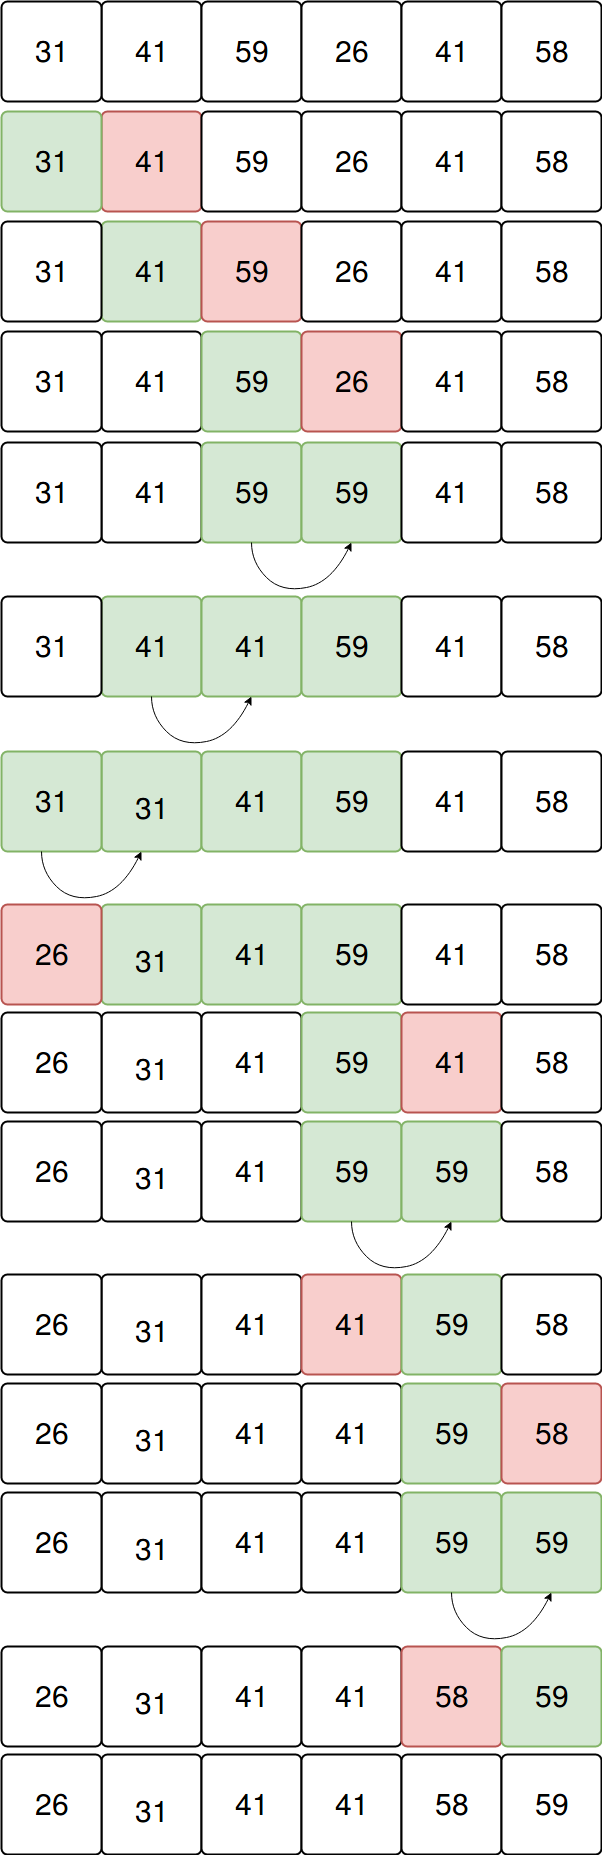
\includegraphics[scale=0.3]{ex-2-1-1.png}\\
  %\footnotesize
  %\vspace{0.10cm}
  %(rodapé da ilustração)
\end{center}
\end{figure}

\newpage

\paragraph{Exercício 2.1-2} Insertion Sort em ordem decrescente (código
completo no repositório GitHub):
\lstset{language=Python}
\begin{lstlisting}[frame=single]
def insertionSort(l):
    for j in range(1, len(l)):
        atual = l[j]
        i = j - 1

        while i >= 0 and l[i] < atual:
            l[i + 1] = l[i]
            i = i - 1

        l[i + 1] = atual

    return print(l)
\end{lstlisting}

\paragraph{Exercício 2.1-3} Busca linear pelo índice onde um número se encontra
em uma lista (código completo no repositório GitHub):
\lstset{language=Python}
\begin{lstlisting}[frame=single]
def buscaNumero(l, n):
    for i in range(0, len(l)):
        if l[i] == n:
            return print(i)
    return None
\end{lstlisting}

Pelo conceito de \emph{loop invariant}, sabemos que a cada iteração de um loop for,
o subarray considerado consiste em todos os elementos originalmente no subarray,
mas ordenados. Assim, no exemplo acima, temos que checar 3 situações:

\begin{itemize}
\item INICIALIZAÇÃO: o \emph{loop invariant} é verdadeiro ANTES da primeira iteração
  loop? Sim, logo após a alocação inicial do primeiro índice do contador (0), e antes
  da checagem do primeiro teste do loop, o \emph{loop invariant} é verdadeiro.
\item MANUTENÇÃO: o \emph{loop invariant} é verdadeiro a CADA ITERAÇÃO do loop?
  Sim, a cada iteração o subarray l[i] consiste do mesmo elemento l[i], trivialmente
  ordenado.
\item TÉRMINO: o \emph{loop invariant} é verdadeiro APÓS o término do loop? Sim,
  pois após o término do loop temos todos os elementos originais.
\end{itemize}

Portanto, podemos afirmar que o algoritmo acima para a busca linear do índice
da localização de um número está correto.

\paragraph{Exercício 2.1-4}

???

%%%%%%%%%%%%%%%%%%%%%%%%%%%%%%%%%%%%%%%%%%%%%%%%%%%%%%%%%%%%%%%%%%%%%%%%%%%%%%%%%%%%%%%%%%%%%%
\subsection{Grupo 2.2:}
\label{grupo_2_2}

\paragraph{Exercício 2.2-1}


%%%%%%%%%%%%%%%%%%%%%%%%%%%%%%%%%%%%%%%%%%%%%%%%%%%%%%%%%%%%%%%%%%%%%%%%%%%%%%%%%%%%%%%%%%%%%%
\subsection{Grupo 2.3:}
\label{grupo_2_3}

\paragraph{Exercício 2.3-1}



%%%%%%%%%%%%%%%%%%%%%%%%%%%%%%%%%%%%%%%%%%%%%%%%%%%%%%%%%%%%%%%%%%%%%%%%%%%%%%%%%%%%%%%%%%%%%%
%%%%%%%%%%%%%%%%%%%%%%%%%%%%%%%%%%%%%%%%%%%%%%%%%%%%%%%%%%%%%%%%%%%%%%%%%%%%%%%%%%%%%%%%%%%%%%
%%%%%%%%%%%%%%%%%%%%%%%%%%%%%%%%%%%%%%%%%%%%%%%%%%%%%%%%%%%%%%%%%%%%%%%%%%%%%%%%%%%%%%%%%%%%%%
%%%%%%%%%%%%%%%%%%%%%%%%%%%%%%%%%%%%%%%%%%%%%%%%%%%%%%%%%%%%%%%%%%%%%%%%%%%%%%%%%%%%%%%%%%%%%%
%%%%%%%%%%%%%%%%%%%%%%%%%%%%%%%%%%%%%%%%%%%%%%%%%%%%%%%%%%%%%%%%%%%%%%%%%%%%%%%%%%%%%%%%%%%%%%
%\newpage
\section{Problemas}
\label{problemas}
%\thispagestyle{plain}


%%%%%%%%%%%%%%%%%%%%%%%%%%%%%%%%%%%%%%%%%%%%%%%%%%%%%%%%%%%%%%%%%%%%%%%%%%%%%%%%%%%%%%%%%%%%%%
\subsection{Problema 2.1}
\label{problema_2_1}

%%%%%%%%%%%%%%%%%%%%%%%%%%%%%%%%%%%%%%%%%%%%%%%%%%%%%%%%%%%%%%%%%%%%%%%%%%%%%%%%%%%%%%%%%%%%%%
\subsection{Problema 2.2}
\label{problema_2_2}

%%%%%%%%%%%%%%%%%%%%%%%%%%%%%%%%%%%%%%%%%%%%%%%%%%%%%%%%%%%%%%%%%%%%%%%%%%%%%%%%%%%%%%%%%%%%%%
\subsection{Problema 2.3}
\label{problema_2_3}


%%%%%%%%%%%%%%%%%%%%%%%%%%%%%%%%%%%%%%%%%%%%%%%
%%% Produz as referências bibliográficas
%% Configura título das referências bibliográficas:
%\newpage
%\renewcommand{\refname}{Referências bibliográficas}
%% Ativa arquivo com as referências bibliográficas:
%\bibliography{evandro}
%% Adiciona entrada na toc:
%\addcontentsline{toc}{section}{Referências bibliográficas}
%% Estilo da página
%\thispagestyle{headings}
%\index{referencias bibliograficas@Referências bibliográficas}


% Termina o documento
\end{document}             
